\section{A New OLED Power Model}
\label{sec:newmodel}

In this section, we present a practical OLED pixel power model that
is more accurate than prior arts and robust to device diversities.

\begin{figure*}[tp]
	\hfill
	\begin{subfigure}[]{0.28\textwidth}
		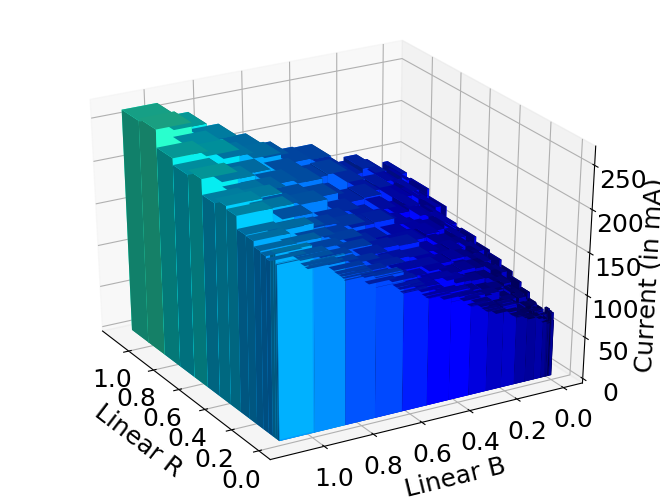
\includegraphics[width=\textwidth]{figure/002_Pixel2_monotonicity_cube.png}
		\caption{Pixel 2}
		\label{fig:initial_monotonicity_n6_w}
	\end{subfigure}
	\hfill
	\begin{subfigure}[]{0.28\textwidth}
		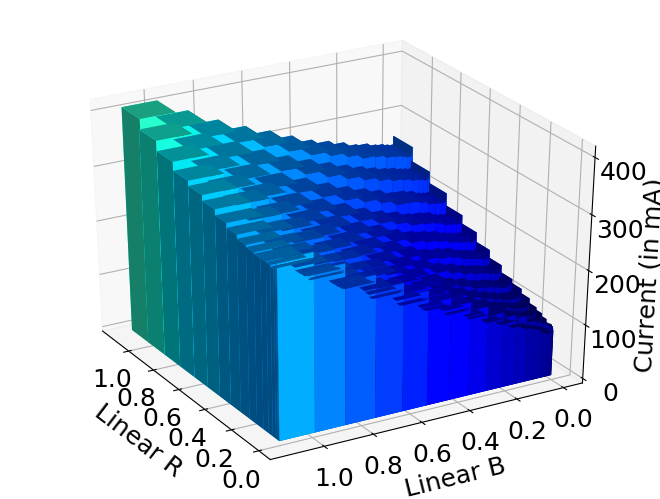
\includegraphics[width=\textwidth]{figure/003_MotoZ3_monotonicity_cube.png}
		\caption{Moto Z3}
		\label{fig:initial_monotonicity_p2_w}
	\end{subfigure}
	\hfill
	\begin{subfigure}[]{0.28\textwidth}
		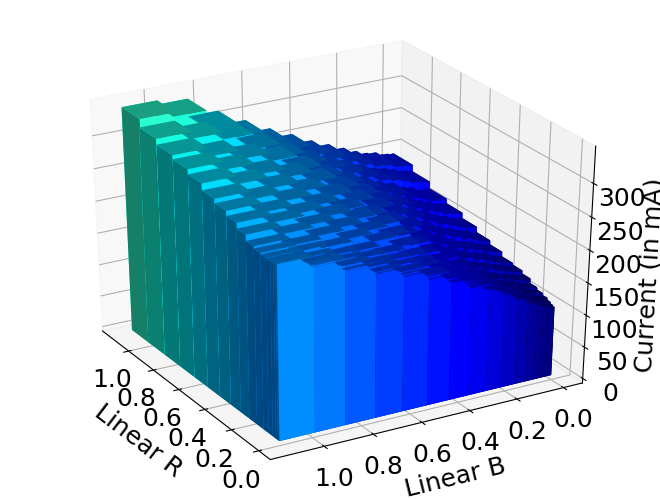
\includegraphics[width=\textwidth]{figure/004_Pixel4_monotonicity_cube.png}
		\caption{Pixel 4}
		\label{fig:initial_monotonicity_z3_w}
	\end{subfigure}
	\hfill
        \vspace{-0.1in}
	\caption{Measured pixel power values for a 2-D dissection of the 3-D color space on the three phones do not fall into a plane.}
\label{fig:initial_monotonicity}
\end{figure*}


\subsection{Key Insight}

Since the non-linear model (NLM) achieves similar accuracy as the linear model
with linear regression (LMLR), 
we discuss our key insight using the
LMLR model.
Recall that LMLR models the pixel power for any given RGB value
$(R_i, G_i,B_i)$ as a linear combination of the subpixel power 
$f(R_{i}), g(G_i)$, and $h(B_i$) (Eqn.~\ref{eq:linear_model_linear_regression}).
%  \begin{equation}
%  	P_i(R_i, G_i,B_i) = e_1\cdot f(R_{i}) + e_2\cdot g(G_{i}) + e_3\cdot h(B_{i}) + e_4
%  	\label{eq:linear_equation9}
%  \end{equation}
Since the subpixel power $f(R_{i}), g(G_i)$, and $h(B_i$) are linear
with respect to the subpixel linear RGB values
(Figure~\ref{fig:initial_evaluation_2}), their linear combination
should be able to and can only fit any plane in the 3-D coordinate space of
($Ri, G_i, B_i$). The question then becomes: do the pixel power values
$P_i(R_i, G_i,B_i)$ fall on a plane?
% in the 3-D color space?

Since it is hard to visualize the measured $P_i(R_i, G_i,B_i)$ in the
3-D RGB space, we select a dissection of the 3-D color space with a fixed
$G$ value (at 112), and plot the measured power value for the 2-D R-B space (in
linear RGB values) in Figures~\ref{fig:initial_monotonicity}(a)-(c) for
the three phones, where the height of the top surface shows the display power
draw values.  We see that the surface is not flat, \ie it does not fall into a plane! This is
the key reason why any particular linear combination of subpixel power functions
(which are linear in the subpixel color) cannot approximate
the pixel power behavior well. In addition,
our experiments in \S\ref{subsec:nonlinear} showed
that adding non-linear terms cannot fit the nonlinear pixel power behavior well either.

We make a key observation that {\em although the pixel power values do not
fall in a plane across the entire color space, they correspond to a reasonably smooth surface,}
\eg as shown in the 2-D dissection example in Figure~\ref{fig:initial_monotonicity}. 
Thus if we cut the 3-D color space into small subgrids, the
pixel power values within each subgrid are likely to fit closely in
a flat plane and thus can be fitted well using linear combinations
of the subpixel (linear) power functions $f(R_{i}), g(G_i)$, and $h(B_i$).

Motivated by the above insight, we propose a new pixel power model
that can estimate the OLED display power with much better accuracy
than the prior art.  The basic idea of the new model is to divide the 3-D
color space (of dimension 256$\times$256$\times$256) into small subgrids
% (\eg of 16$\times$16$\times$16 sRGB values each)
and derive a piecewise LMLR model for each subgrid.

% \begin{equation}

% \begin{bmatrix}
%     y \\
%     m \\
%     c \\
%     w
% \end{bmatrix}
% =
% \begin{bmatrix}
%      0.544 &      1.489 &      0.000 \\
%      0.638 &      0.000 &      1.000 \\
%      0.000 &      1.193 &      0.739 \\
%     -0.201 &      4.125 &     -0.401
% \end{bmatrix}

% \end{equation}


\subsection{Model Derivation}
\label{subsec:modelderivation}

% Piecewise model (in RGB space)
% Linear (3 var vs. 4 var)
% Non-linear (8 var) <r+g+b+rg+bg+gr+rgb+c>
% precedural

Deriving the above piecewise pixel power model consists of three
steps: decomposition of the color space, data collection, and model
derivation for each sub color space.

\begin{figure}[tp]
	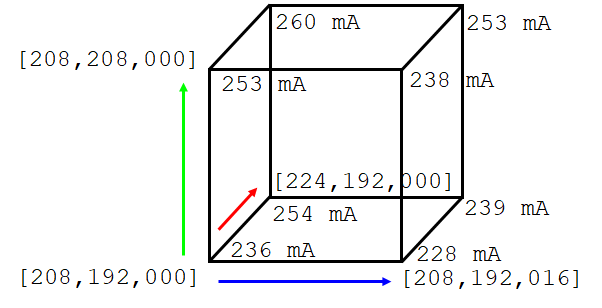
\includegraphics[width=0.35\textwidth]{./figure/004b_Cube_Model.png}
        \vspace{-0.1in}
	\caption{A 16$\times$16$\times$16 subgrid in the 3-D sRGB color space.}
        \vspace{-0.15in}
	\label{fig:cube_model}
\end{figure}
%   \begin{figure}[]
%   	\includegraphics[width=0.45\textwidth]{./figure/005_Cube_Zoom.png}
%   	\caption{How the cube in color space segmentation looks like.}
%   	\label{fig:cube_zoom}
%   \end{figure}


First, we decompose the 256$\times$256$\times$256 RGB color space into
subgrids of size $s\times$$s$$\times$$s$, where $s$ is the granularity of
the piecewise pixel power model. The choice of $s$ determines the
tradeoff between accuracy and the model size. The model size in turn
determines the memory and lookup
overheads. Figure~\ref{fig:cube_model} shows an example grid
of size 16$\times$16$\times$16 resulted from decomposing the
3-D color space into 16$\times$16$\times$16 subgrids.

Second, we experimentally measure the pixel power value as before
(\S\ref{subsec:super}) by displaying monochromatic images one at a time
corresponding to the color of each grid point in the decomposition. For
$16\times 16 \times 16$ subgrids, there will be $17^3 = 4913$ grid
points.

Finally, for each subgrid, we derive a pixel power model by applying linear regression 
to derive the coefficients of the model, \ie by fitting the power values at its 8 corner grid points
(see Figure~\ref{fig:cube_model}).  We
evaluate two model types for each subgrid, LMLR
(Eqn.~\ref{eq:first_order_variable}) and NLM (Eqn.~\ref{eq:second_order_variable}),
and denote the new models as P-LMLR (piecewise LMLR) and P-NLM (piecewise NLM):

\vspace{-0.1in}
{\small
  \begin{align}
	P^{grid_j}_i &= e_1^j\cdot f(R_i) + e_2^j\cdot g(G_i) + e_3^j\cdot h(B_i) + e_4^j
	\label{eq:first_order_variable} \\
  P^{grid_j}_i &= e_1^j\cdot f(R_i) + e_2^j\cdot g(G_i) + e_3^j\cdot h(B_i) + \label{eq:second_order_variable} \\
&  e_4^j\cdot f(R_i)g(G_i) +
  e_5^j\cdot f(R_i)h(B_i) +
  e_6^j\cdot g(G_i)h(B_i) +
  e_7^j \nonumber
\end{align}
}
\noindent
%The reason we add constants $e_4^j$ and $e_^j$ is because the power odes not start from

\vspace{-0.1in}
\paragraph{Handling color transformation.}
{For the cases with color transformations, \ie due to 
% brightness level change,
%(on Pixel 2 and Moto Z3)
color mode change or color correction,
 if  the color transformation, \ie the color matrix, is known,
 the new power model can be derived from the default power model;
 otherwise, the new power model needs to be experimentally generated.
}
% This is because the hardware composer changes the colors
% in hardware, which is in perceivable to the software.}

\if 0
Second major design aspect is to compute the OLED display current withing
16.7 ms. For this purpose we considered sampling of the image and found that
the relative error is small with sampling as seen in the
Figure\ref{fig:smaplinh_error}. The time taken for computation with various
sampling rates are shown in Figure\ref{fig:smapling_time} and we concluded
that even with sampling of less than 1\% we can get low relative error with
computation speed up. However to get the complete data for a full resolution
image it can take up to 2.5 seconds which is no where in our required limits
of 16.7 ms.
\fi

% \subsection{Model Design and Application}

% Model derivation
% training
% Using model online
% Memory-efficient sampling
% Table lookup the piecewise model
% Overhead evaluation

\if 0
\subsection{Model Training}

We created an android app which displays a mono-color image. This mono-colored
image corresponds to the edge of the cube explained above. R language was used
to generate the 4 variable linear equation to estimate power for each cube.

When deriving the power for the OLED display,we sampled 1\%  of the screen.
For each sampled pixel the matching color cube is selected and corresponding
equation is used to estimate the current consumed by the pixel. 
The current (power) is added up and extrapolated to obtain  the current for
the full screen.

We created an utility using OpenGL call to generate a virtual display.
The overhead to generate the virtual display is less than 5 ms per frame with a
power overhead of {TODO:power overhead J for Nexus 6, x J for
Moto Z3 and x J for Pixel 2.}
\fi



\subsection{Using the Model in Real Time}
\label{subsec:appl}

Using the new OLED power model in real time includes four simple steps:
(1) Record a pixel frame, \eg via a virtual display,
% we can estimate its OLED power draw in three simple steps:
(2) For each pixel in the frame, find the sRGB subgrid it belongs to;
(3) Apply the piecewise pixel power model of that subgrid to
estimate the power draw for the pixel;
(4) Sum up the estimated power for all the pixels
(Eqn.~\ref{eq:linear_equation0}).

\if 0
\dcomment {
On the same three phones,
once a frame is recorded in memory, Steps 2--4 only take
10ms, 10ms, and 4ms, respectively.  However, we found recording a single frame from
the virutal display can easily take hundreds of milliseconds, which
prevents the model from being used in real time, \eg by an
enhanced Android Battery (\S\ref{subsec:tool2})}

%  can incur significant computation overhead as modern
%  OLED displays come with millions of pixels.  {For example, the Nexus 6
%  OLED display has 8 million pixels, and calculating the power for
%  every pixel using the LMLR model in our highly optimized C
%  implementations takes 1 second on a Dell laptop.  }


To control the frame recording time to be a fraction of the 16.7ms
per-frame rendering time,
we apply uniform pixel sampling (experimentally found to be faster than random sampling
yet give similar modeling accuracy) similarly as
in~\cite{dong2009current}.
We define {\em sampling ratio $K$} as the factor of reduction: one pixel is chosen from
the center of each grid of
$\sqrt{K}\times\sqrt{K}$ pixels.
The choice of the sampling ratio determines the tradeoff between
runtime reduction and modeling error.
We experimentally evaluate the tradeoff in the next section. NOT CORRECT. WAS RELEVANT IN NEXUS 6
\fi

{
On the same three phones,
% once a frame is recorded in memory,
Steps 1--4 takes
54ms, 58ms and 46ms, respectively.
This prevents the model from being used in real time, \eg by 
enhanced Android Battery (\S\ref{subsec:tool2}).
% \comment{
% However, we found recording \comment{and accessing} a single
% frame from the virtual display can easily take hundreds of milliseconds,
% which prevents the model from being used in real time, \eg by an
% enhanced Android Battery (\S\ref{subsec:tool2}).
% REMOVING THIS
% }
To control the execution time of Steps 1--4 
% frame recording time
to be within a fraction of the 16.7ms, \ie per-frame
rendering time, we apply uniform pixel sampling (experimentally found to
be faster than random sampling yet gives similar modeling accuracy) similar as 
in~\cite{dong2009current}. We define {\em sampling ratio $K$} as the factor
of reduction: one pixel is chosen from the center of each grid of
$\sqrt{K}\times\sqrt{K}$ pixels. The choice of the sampling ratio determines
the tradeoff between runtime reduction and modeling error. We experimentally
evaluate the tradeoff in the next section.
}

\if 0
\subsubsection{A user-level online tool}

An android app was created which can train itself for any phone which is equipped with an
OLED display. Once the OLED model is generated the app will give a real time display
power estimate on the screen. The current update of the power is kept at 1 sec but it can
be change to 60 time a second to match the 60 FPS display of the modern phone display.
\fi


%%%%%%%%%%%%%%%%%%%%%%%%%%%%%%%%%%%%%%%%%%%%%%%%%%%%%%%%%%%%%%%%%%%%%%%%%%%



\if 0
\subsection{Fast Modeling for Profiling a Single Frame}
\label{subsec:fast}

On newer phones such as Pixel 2 and Moto Z3, the built-in power sensor has a low
sampling rate, at approximately every 1.4 seconds. With this sampling rate,
the model generation process in \S\ref{subsec:modelderivation} will take approximately 12 hours for 4096
piecewise models and 1.4 hours for 512 piecewise models.
Though model generation is a one-time effort,
it can be too long for first-time use of the power model.
Furthermore, an app designer often has to test her app on various
devices before releasing the app, each requiring its own model generation.
%  So modeling and optimizing app in various devices is very time
%  consuming given that for a UI design consists of a small proportion of
%  colors.
We discuss a quick way of model generation, which can be used
in modeling the OLED power draw of a single frame on a new device.
%% \comment{factor of 8 dfference?}
%% This is because ???
%  This is because to ensure the experiment very
%  precisely during the long test duration, \ie the external
%  environmental conditions like temperature.

We observe that for the set of apps we experimented with (listed in
\S\ref{tab:experiments}), if we plot the histogram of the pixel colors
in the activity frames, a few distinct peaks (??to ???) account for a majority of
the frame pixels. This happens because the app activity UIs are
synthetically colored, and the app developer tends to use just a few colors
in the design. The remaining pixels have many colors spread in the
histogram with low frequencies which come from dynamic objects (\eg
images) in the frame which tend to have continuous textures.

%   the histogram is very distinct and has few peaks i.e. about 0.2\% of
%   the total number of images used to generate 16x16x16 model and 1.6 \%
%   of 32x32x32 model.  This shall take less than 2 minutes for the apps
%   as compared to hours for generate the complete model.


%  When designing the UI, the developer will not consider these
% objects as these are updated at the runtime.

Our fast model generation derives pixel power needed for modeling such
a typical frame as follows. First, we detect UI components in the frame to
identify dynamic components. We do this by using the Per-Frame OLED Power 
Analyzer (described in \S\ref{subsec:analyzer}).  Second, we generate the histogram
pixel colors to identify the peaks that correspond to the colors used
in the UI design. Third, we derive the pixel power draw for each of the few peak colors
following the methodology in \S\ref{sec:measurement},
each of which takes only 10 seconds. Finally,
we use the pre-generated simple LMLR model (dervied from four basic pixel colors)
to model the power draw of remaining pixels.
Though the LMLR model can be inaccurate, since it is only used for a small percentage of pixels,
\comment{what is the dynamic content is big???}
its error with respect to total display current will be very small.

\fi



\if 0
There might be some continuous components in the activity which may not contribute
to more than 1\% like the shadowing of the text. For this we switch to the linear model.
As we have seen earlier we estimate the red, blue and green curve in linear RGB,
by only knowing the lowest and highest intensity current. So in total for this we
require 4 (as the lowest intensity in all red, green and blue is black) images to evaluate the current.
The error in linear model is high but it will be a small fraction of the screen and
this error with respect to total display current will be very small.

We generate the histogram of the entire screen. We find all peaks which have
a contribution to the screen area more than 1\% of the screen area.
\fi

\if 0
\subsubsection{Implementation:}
We created an Android app for this purpose.
We brought the Android screencap command. We fetch
the screen and generate an histogram.
We identify the peaks. We go into a app training mode where the model is evaluated
by displaying monochromatic images on the screen. Each of the image is shown for 5 to 10
seconds.
If the peaks do not cover 99\% of the screen , we also calibrate 4 more images i.e.
black, read, green and blue at full intensity for linear model.
\fi


